\newcommand{\kcomment}[1]{{\color{blue}{#1}}}

\section{The problem}

In \emph{patrolling} problems, one or more agents move around a given terrain to defend or supervise it by visiting designated places in the terrain with sufficient frequency~\cite{czyzowicz2011boundary}. 

Here we consider the problem where the terrain is represented by an undirected graph with specified edge lengths, on which agents move with speed $1$ or less.  Each vertex has an \emph{idle time}, and is said to be \emph{guarded} by a set of moving agents if it is visited at least once in every time period of that length.  We are interested in deciding whether there is a schedule for a given number of agents to guard all vertices. 

Since the problem for general graphs is NP-hard even for a single agent, we consider the following special graphs: \emph{lines} (paths), \emph{stars} and \emph{unit-length cliques}. 
A star is a graph where there is a special vertex called the \emph{centre}, 
which does not need to be guarded,
and all other vertices are adjacent only to the centre. 
A unit-length clique is a complete graph with all edges equal in length. 
Since all that matters for patrolling is the time it takes to travel between each pair of nodes, a unit-length clique can be regarded as a special case of a star with all edges equal in length. 

\section{Previous work with no cooperation}

Coene et al.~\cite{coene2011charlemagne} studied a slightly different version of the problem which require that each vertex be guarded already by one agent alone.  In this setting, they showed polynomial time algorithms and NP-hardness results for some graph classes. 
We remove this requirement and study the problem where a vertex can be guarded by several agents in cooperation.

%% (conditions of security)
%% (uncooperative) \kcomment{←これらの言葉を使うなら単に括弧内に記すのではなく説明せよ。でも結局この原稿中では後で使うわけではないようですね(???最後の節で前者が出てきているが)。}

%% \kcomment{↓「Unit」などはグラフの名なのか、グラフの集合の名なのか、入力をそれに制限した問題の名なのか。どれでもよいがはっきりさせよう。}

The two versions of the problem come to the same thing when there is only one agent.
For this setting, Coene et al.~\cite{coene2011charlemagne} gave 
polynomial time algorithms for trees with uniform idle times and for lines, 
and proved that the problem is NP-hard for stars with arbitrary idle times.
Thus, our study of the cooperating agents will focus on the cases where the problem is not already known to be NP-hard for single agent, that is, for (1) lines, (2) unit-length cliques, (3) stars with uniform idle times.
% , and (4) trees with uniform idle times.

\begin{figure}[htbp]
  \begin{tabular}{cc}
    \begin{minipage}{0.5\hsize}
      \centering
      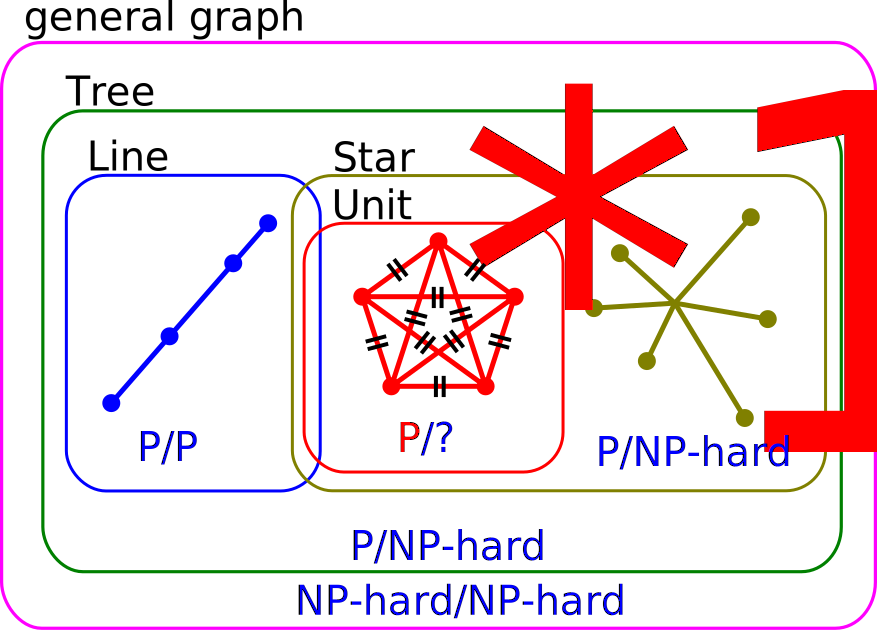
\includegraphics[width=\hsize]{../fig1_adjust.pdf}
    \end{minipage}
    \begin{minipage}{0.5\hsize}
      \centering
      \includegraphics[width=\hsize]{../fig2_adjust.pdf}
    \end{minipage}
  \end{tabular}
  \caption{Classes of graphs and the complexity of the patrolling problem.
  The left figure is for a single agent and the right figure is for multiple agents in cooperation.
  The left side of the slash represents the case of uniform idle times, and the right side represents the case of arbitrary idle times.}
  \label{fig:shapeandcomplexity}
\end{figure}




\section{Uniform idle time}
%% For each graph, we first considered the case where all vertices have the same idle time.  We proved that all of them \kcomment{(←何を指す?「lineでもstarでも」という意味?)} can be calculated in polynomial time.
We first considered the case where all vertices have the same idle time.  We proved that our problem can be solved in polynomial time both for lines and for stars, because in these cases the situation is simplified in the following way: 
For lines, we showed that if patrolling is possible at all, then there is a patrolling schedule where each vertex is guarded by one agent alone. 
For stars, there is a schedule where the only form of cooperation is for several agents to periodically visit a subset of vertices in the same order at a certain time interval.

% In this way, it was found that if the cooperation of the agents is unnecessary or when the cooperation method becomes extremely simple due to all equal allowable visiting intervals, it \kcomment{(←何を指す?)} can be easily solved.
% ↑節の冒頭第二文で述べたことにしました。
For these graphs, we can also efficiently solve the optimization problem where each vertex has a profit and we want to maximize the sum of the profit of the guarded vertices. 

\section{Arbitrary idle times}

On the other hand, because it was difficult to evaluate the complexity class of lines and unit-length cliques when idle time was general, we considered
% \emph{visit time designation} as a condition instead of idle time.
another condition different from idle time for being guarded.
% \kcomment{←どういう意味?(複数の文が途中で混ざっている?)「訪問時刻指定」の説明をしようとしている?}
As a result, we found an algorithms that greedily determine the motion of the agent in lines (Figure \ref{fig:shapeandcomplexity}-*2 ).
% \kcomment{(ここの間に「一方で利得最大化問題を考えると」という説明が要りますよね?)}
Furthermore, it was shown that
the optimization problem also mentioned at the end of section 3 for unit-length cliques is NP-hard by a reduction from the maximum independent set problem
(Figure \ref{fig:shapeandcomplexity}-*1 ).
